\documentclass[coverheight=210mm,coverwidth=148.5mm, bleedwidth=13mm,
spinewidth=13mm, foldingmargin, marklength=4mm, 11pt]{bookcover}

\usepackage[utf8]{inputenc}
\usepackage[spanish,es-tabla]{babel}
\usepackage{microtype}
\usepackage{qrcode}
\usepackage[outline]{contour}
\contourlength{.5pt}

\usepackage[sc]{mathpazo} % Use the Palatino font with smallcaps
%\usepackage[osf]{mathpazo} % Palatino with smallcaps and oldstyle numbers

% \usepackage{avant} % Avant Garde Sans Serif
% \usepackage{helvet}
%\usepackage{tgadventor}
%\usepackage{AlegreyaSans}
\usepackage{biolinum}
%\usepackage{fetamont}
\usepackage{eulervm} % Euler math


\usepackage[T1]{fontenc}
\usepackage{microtype}

\definecolor{openscadyellow}{HTML}{FFFFE5}


\begin{document}

\begin{bookcover}

   \begin{bookcoverelement}{color}{bg back}
     openscadyellow
   \end{bookcoverelement}
   \begin{bookcoverelement}{color}{bg spine}
     openscadyellow
   \end{bookcoverelement}


  \begin{bookcoverelement}{center}{back}
    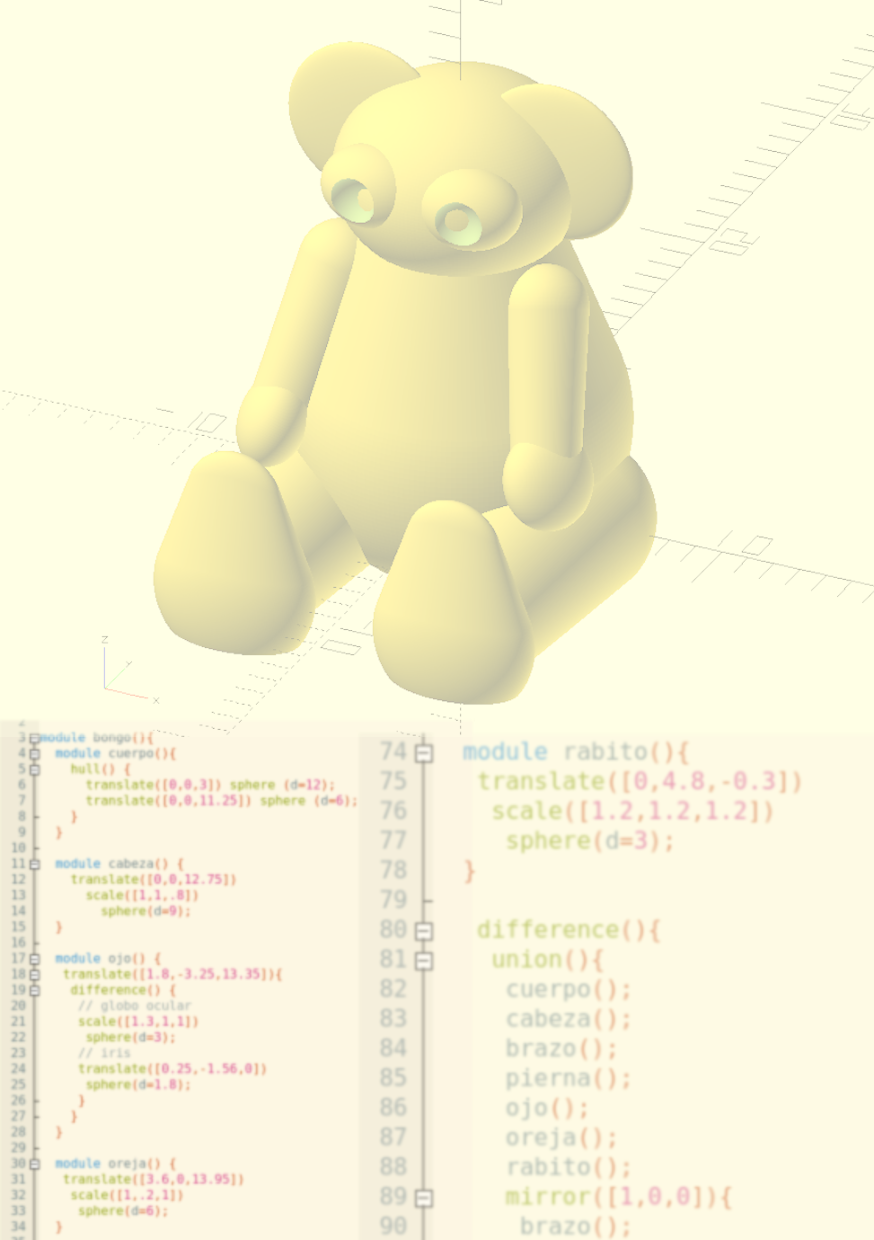
\includegraphics{contratapa-A5.pdf}
  \end{bookcoverelement}


  \begin{bookcoverelement}{normal}{back}[1.5cm,2cm,2cm,1cm]
    {\large

      \hspace{.5em} [...] Cecilia pensó que Antonia tenía
      razón. El objeto que tenía entre sus manos y que volvía y
      revolvía en ellas era muy hermoso; tanto más que aún no lo
      comprendía del todo y por lo tanto estaba cargado con todas las
      promesas del misterio y las posibilidades de la
      geometría. <<Este objeto>> ---pensó Cecilia--- <<será infinito
      mientras no lo comprenda del todo>>. No obstante, sabía que la
      pulsión por entender la vencería, y la finitud se cerniría sobre
      ese semicilindro de plástico que sus dedos acariciaban.

      \hspace{.5em} ---¿No me vas a preguntar cómo lo hice? ---Antonia
      hizo pucherito, simulando contrariedad y sonriendo con los ojos.

      \hspace{.5em} Cecilia salió con una sonrisa de su
      ensimismamiento y se dispuso a escuchar. [...]
  

  \begin{flushright}
    \emph{Fragmento del capítulo 3}
  \end{flushright}

  \vspace{2.5em}
  
  \hspace{.5em} [...] ---No parece un problema muy difícil de resolver
  ---a\-ven\-tu\-ró Cecilia---; supongo que deberemos escribir dos
  relaciones matemáticas entre horas y ángulos: una para cada
  hemisferio. Y permitir que el usuario indique, mediante una
  variable, si desea usar su reloj en el norte o en el sur, y en
  función de eso emplear una u otra relación: suena a una tarea para
  un \texttt{if}.

  \hspace{.5em} Antonia sonreía mientras escuchaba y caminaba junto a
  Cecilia. Pensó que ya empezaba a sonar como una programadora:
  elevando suposiciones al rango de algoritmos, cifrando sentencias
  breves al borde de lo confuso, y hasta enfrentando problemas aún no
  resueltos con una confianza demasiado parecida a la pedantería. Por
  un momento temió estar echándola a perder; pero decidió que, en
  cualquier caso, ya era demasiado tarde. [...]

  \begin{flushright}
    \emph{Fragmento del capítulo 23}
  \end{flushright}
}
  
  \end{bookcoverelement}


\end{bookcover}

\end{document}
